\newsection
\subsection{BP 1: Single wave on a simple beach (Analytic)}

{\bf Documentation:} 
\begin{itemize}
\item A description of this benchmark problem is provided by \cite{bp-description} and \cite{SynolakisBernard:pmel135}.

\item Problem description provided by Dmitry Nicolsky, 
at \cite{bp-description}: \\
\href{https://github.com/rjleveque/nthmp-benchmark-problems/blob/master/BP01-DmitryN-Single_wave_on_simple_beach/description.pdf}
{BP01-DmitryN-Single\_wave\_on\_simple\_beach/description.pdf} 
\end{itemize} 

\subsubsection{Problem Description}
The focus is on comparing computed and analytic solutions for a wave incident on a simple beach, in which:
\begin{itemize}
\item The bathymetry consists of a deep region of constant depth $d$
connected to a sloping beach of angle $\beta = \text{arccot}(19.85)$. 
Note that the toe of the beach is located at $x = X_0 = d \text{cot} \beta$
\item The initial waveform of the wave is given by 
\begin{equation}
\eta(x,0) = H \text{sech}^2(\gamma (x - X_1)/d)
\end{equation}
where $L = \text{arccosh}(\sqrt(20))/\gamma$, $X_1 = X_0 + L$, 
and $\gamma = \sqrt(3H/4d)$. The speed of the wave is given by the following: 
\begin{equation}
u(x,0)=-\sqrt{g/d}\eta(x,0)
\end{equation}
\end{itemize}

\begin{figure}[ht]
\hfil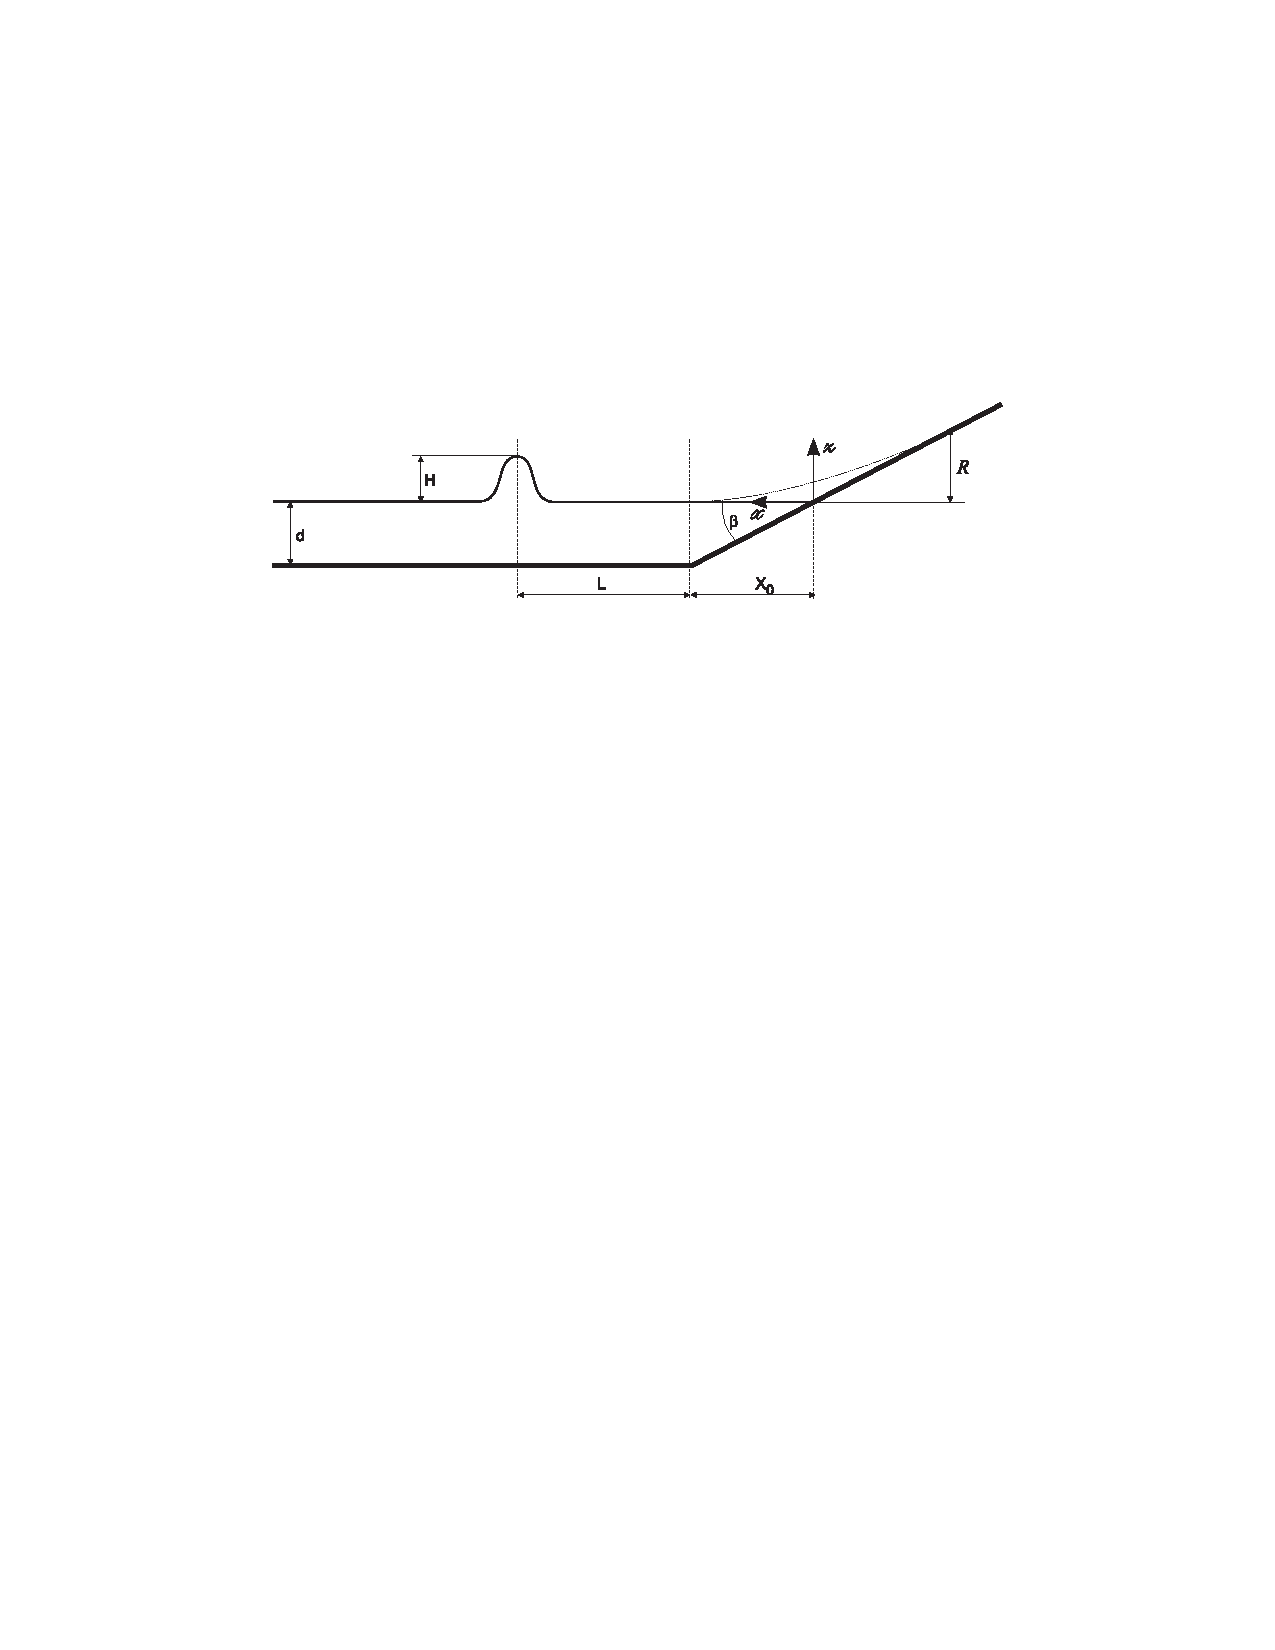
\includegraphics[width=5.0in]{bp1/bp1domain}\hfil
\caption{\label{fig:bp1domain} 
Sketch of canonical beach and approaching wave.
 }
\end{figure}


\subsubsection{Problems encountered}

\begin{itemize}
\item The analytic solution of the wave equation was hard to determine and compute.  The analytic solution was obtained from the benchmark problem champion; it would be very helpful if it were provided in an Excel file as part of the benchmark problem description.  
\item No analytical solution was provided for time $t = 25s$
\item The Clawpack code does not currently include maximum runup calculations. An additional module had to be written. 
\end{itemize}

\subsubsection{What we did}

\begin{itemize}
\item Used $g=1$ and no friction.
\item The problem was solved on an $800\times 2$ grid, where the x domain spanned x = -10 to 60.
\item Variable time stepping was allowed, based on a CFL number of 0.9
\end{itemize} 

\subsubsection{Results}
\begin{itemize}
\item Task 1. Good agreement between computed and analytic water level profiles at $t = 35(d/g)^{1/2}$, $t = 45(d/g)^{1/2}$, $t = 55(d/g)^{1/2}$, $t = 65(d/g)^{1/2}$ is presented in Figure \Fig{bp1frames}.  Data were missing from file {\tt canonical\_profiles.txt} for $t=25(d/g)^{1/2}$, so this time was omitted.
\item Task 2. Good agreement between computed and analytic water levels at locations $x/d = 0.25$ and $x/d = 9.95$ during the propagation and reflection of the wave is presented in Figure \Fig{bp1gauges}.
\item Task 3. Maximum runup on the beach was 0.085, as presented in the time series of runup values in Figure \Fig{bp1runup}.
\item Task 4. The optional demonstration of convergence was not performed.
\end{itemize}

\begin{figure}[ht]
\hfil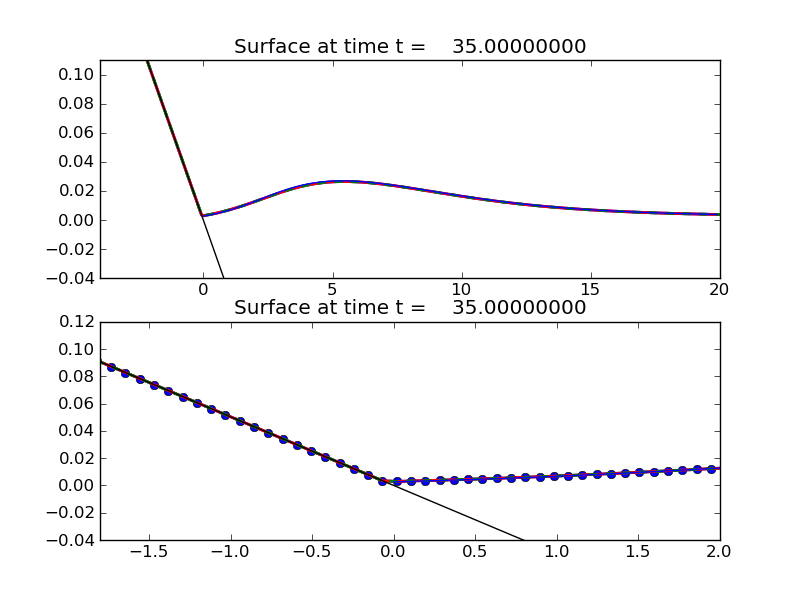
\includegraphics[width=2.8in]{bp1/frame0001fig2.png}\hfil
\hfil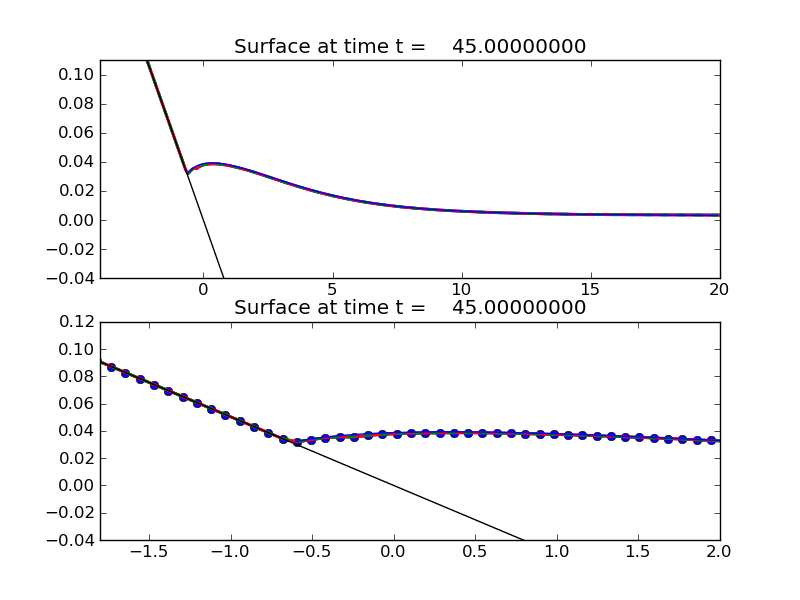
\includegraphics[width=2.8in]{bp1/frame0003fig2.png}\hfil
\vskip 5pt
\hfil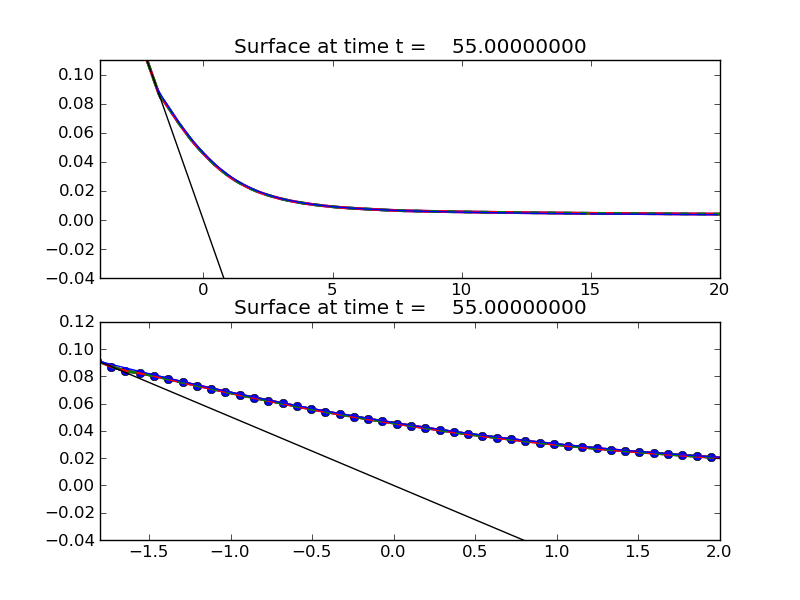
\includegraphics[width=2.8in]{bp1/frame0005fig2.png}\hfil
\hfil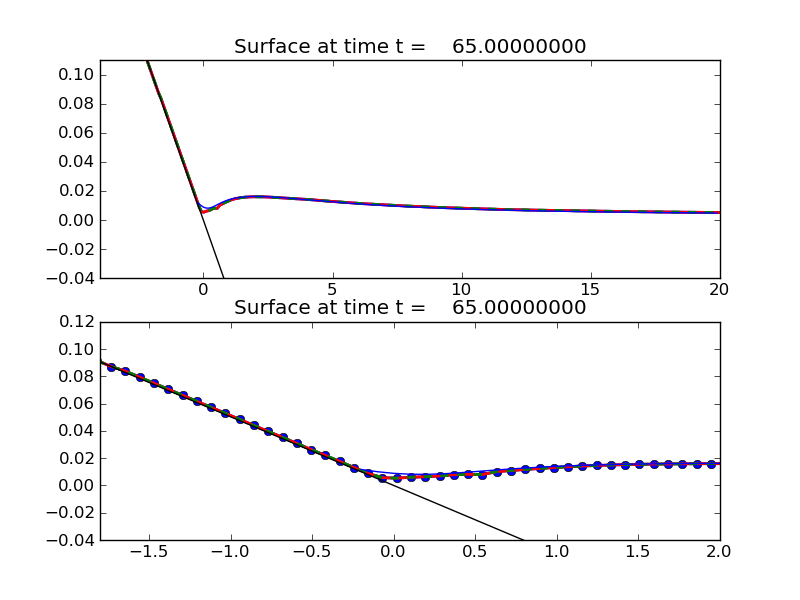
\includegraphics[width=2.8in]{bp1/frame0007fig2.png}\hfil
\caption{\label{fig:bp1frames} 
Profile plots for the times specified in Task 2.  For each pair of plots at a particular time, the top frame provides a full view of the incoming wave and the bottom frame provides an expanded view of the inundation area. In some regions the analytic and GeoClaw solutions lie atop one another.
\todo{Redo plots with only two lines?  Currently several curves are
all the same.}}
\end{figure}

\begin{figure}[ht]
\hfil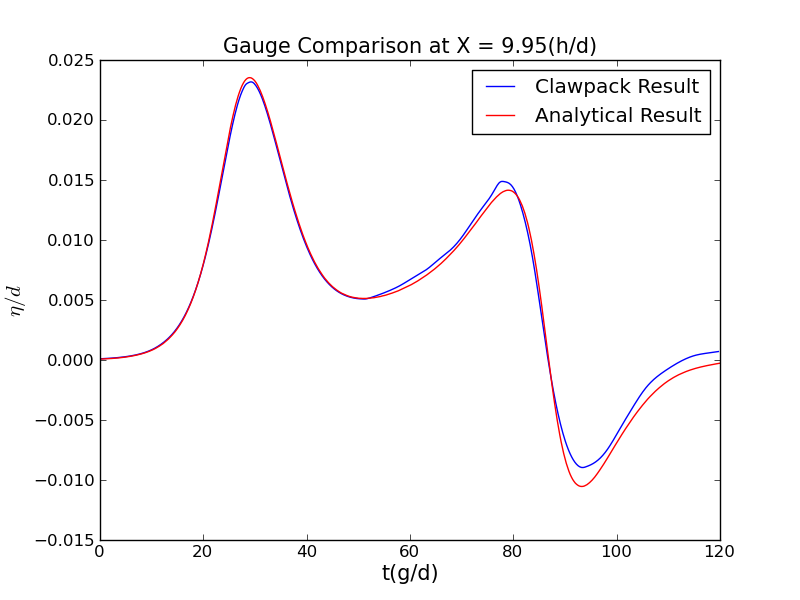
\includegraphics[width=2.8in]{bp1/plotgauge2.png}\hfil
\hfil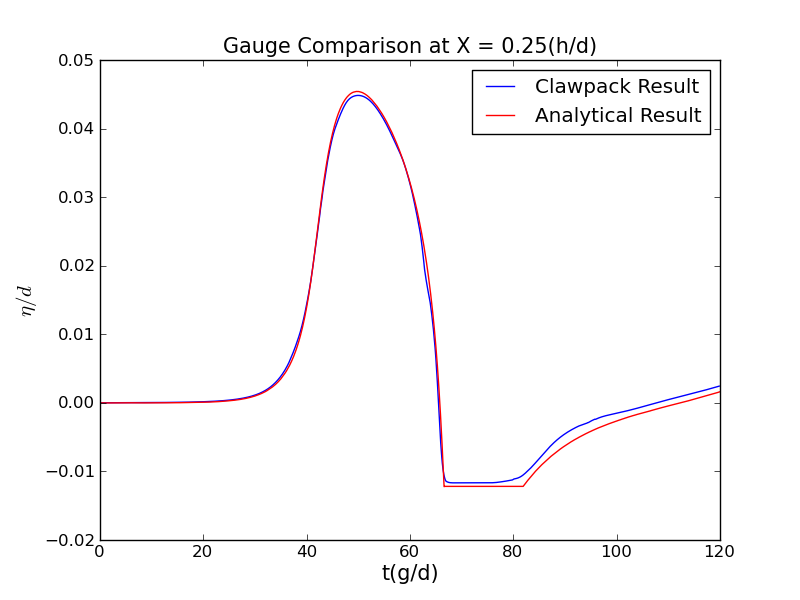
\includegraphics[width=2.8in]{bp1/plotgauge1.png}\hfil
\caption{\label{fig:bp1gauges} 
Left column: Water level time series at location $x/d = 9.95$.
Right column: Water level time series at location $x/d = 0.25$.
 }
\end{figure}

\begin{figure}[ht]
\hfil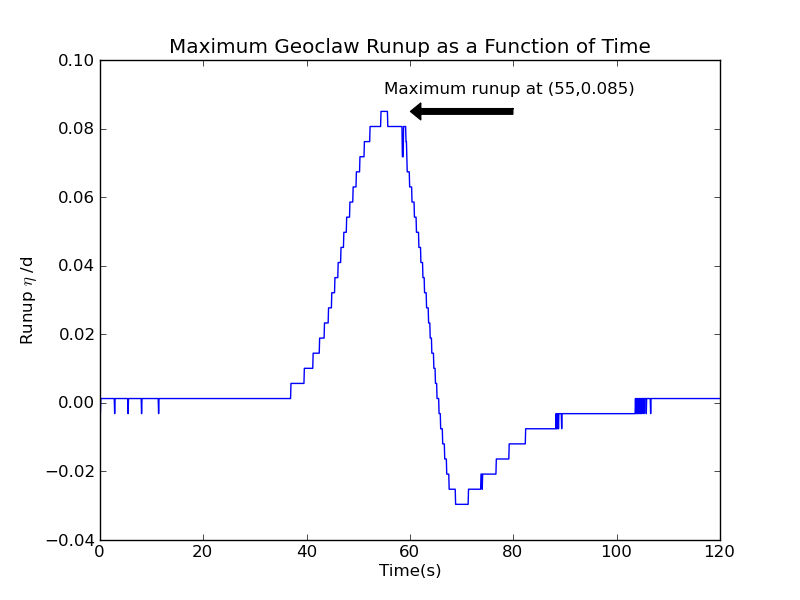
\includegraphics[width=5.5in]{bp1/runup.png}\hfil
\caption{\label{fig:bp1runup} 
Runup on canonical beach as a function of time}
\end{figure}

\subsubsection{Lessons learned}

\begin{itemize}
\item This benchmark problem is a good test of the shallow water wave computation against an analytic solution in one dimension.
\item Because of its complexity, the analytical solution should be provided in a data file on the benchmark problem website to ensure all participants are solving the same problem.
\end{itemize}
